\section{Evaluation}\label{sec:experiments}

In our evaluation, we wanted to understand the effect of batching and reordering, the performance of our validator reordering algorithms as well as different policies, and the impact of parallelization at the validator.
% as well as configuration parameters. In particular, 
We wanted to answer the following questions:
\changed{
\begin{enumerate}[leftmargin=*, nolistsep]
\item 
	How well do our validator reordering algorithms from Section~\ref{subsec:validator_reordering:algorithm} perform? How do these algorithms affect the end-to-end system performance? (Section~\ref{sec:exp_algorithms})
%\vspace{-0.5em}
%(2) What is the impact of batch size on performance? 
\item How does storage and validator batching and reordering
  affect system performance? (Sections~\ref{subsec:experiment:batching} and~\ref{subsec:experiment:smallbank})
%\vspace{-0.5em}
\item How do different policies from Section~\ref{subsec:validator_reordering:policy} impact performance? (Section~\ref{subsec:experiment:policy})
%\vspace{-0.5em}
\item How do we incorporate our techniques on top of a state-of-the-art OLTP system and a commercial database, and what is the resulting performance? (Sections~\ref{sec:OtherOLTP} and~\ref{subsec:experiment:compare})
\end{enumerate}
Table~\ref{tbl:exp} summarizes the settings we evaluated and describes the tradeoff encapsulated in each parameter. 
We also describe parallelization of our algorithms in detail in Appendix \ref{sec:parallel} and 
show the resulting benefits in Appendix~\ref{sec:experiments:parallel}.
% Appendix~\ref{sec:parallel}.
}
%\vspace{-0.5em}
%\item How does parallel reordering affect performance?

\begin{table*}[h]
	\centering
\changed{
		\captionof{table}{\changed{Summary of settings and trade-offs}}
	\begin{tabular}{|c|c|}
		\hline
		{\bf Setting} & {\bf Trade-off} \\
		\hline
		Batch size & Larger batch sizes give more flexibility of reordering but can increase transaction latency. \\
		\hline
		FVS algorithms & The sort-based algorithm is cheaper but includes more transactions in the FVS. \\
		\hline
		Minimize aborts & Reorder transactions to reduce the number of aborts.\\
		\hline
		Minimize tail latency & Reorder transactions to reduce tail latency at the cost of slightly increased aborts.\\
		\hline
		Reduce inter-thread conflicts & Reorder transactions to achieve thread locality for decentralized system architecture. \\
		%for decentralized multi-threaded OLTP architectures based on OCC.\\
		\hline
	\end{tabular}
	\label{tbl:exp}
}
\end{table*}


\subsection{Experimental Setup}
\label{subsec:experiment:implementation}

%Our system architecture consists of four components: a transaction client, a processor thread, a storage thread, and a validator thread. The threads communicate through queues of requests; that is, there is a generator queue, a processor queue, a storage queue, and a validator queue.

\changed{We first describe the experimental setup for our research prototype where we isolate the impact of different parameters in our algorithms. Section~\ref{sec:OtherOLTP} and~\ref{subsec:experiment:compare} describe our experiments with an open-source OLTP system and a commercial database system; both of these sections will describe their own experimental setups respectively.}

Our \changed{research prototype system architecture} has four components: Transaction clients, processors, storage, and a validator as shown in Figure~\ref{fig:occ_arch}. The components communicate through consumer-producer queues. 
The transaction client continuously produces new transactions until the system reaches the maximum permitted concurrency level. The processor acts as a transaction coordinator and \emph{multiplexes} multiple transactions in parallel. It receives transaction requests from clients, sends read/write requests to the storage, sends validation requests to the validator, restarts aborted transactions, and replies commit messages to clients.\cut{ It also restarts aborted transactions so that it only communicates commit decisions to the transaction client.}

The processor is \emph{non-blocking}: It processes requests from its consumer-producer queue without waiting for the response of the request. For example, when it receives a transaction request from a client, it sends read requests on behalf of this transaction to the storage, and then it continues to process the next request in its queue without waiting for the response from the storage. This asynchronous processing allows the processor to multiplex many transactions in parallel to improve its throughput.

The storage processes read and write requests. With storage batching, the storage buffers requests into batches and processes the requests as described in Section~\ref{subsec:storage_reordering}.\cut{first execute all the write requests and then all the read requests in the batch.}

% validator
The validator performs backward validation. For every transaction, a validation request consists of the keys and versions of its reads and the keys of its writes. The validator caches the write keys of committed transactions in an in-memory hash table, until these writes are overwritten by later updates.
We have decoupled the validator into three components as described in Section~\ref{subsec:validator_reordering}. A batch preparation worker receives validation requests from the processor, packages transactions into batches, and sends them to transaction reordering workers. A transaction reordering worker pre-validates all the transactions in the batch against the current state of the validator cache, reorders the transactions, and sends ordered transactions to the validation workers. A validation worker processes batches of \changed{transactions} one by one. It validates transactions against the current validator cache and applies updates from committed transactions to the cache based on the transaction serialization order.  When batching is enabled, the validator collects the requests into a batch as they arrive, and runs one of the algorithms from Section~\ref{subsec:validator_reordering:algorithm} to determine a serialization order. Every transaction that passes the validation is assigned an integer \emph{commit timestamp}, which corresponds to the version number of the updates it will install in storage. 
% Details of validator implementation.
By default, the validator uses the sort-based greedy algorithm with the \texttt{prod-degree} policy and multi factor  value $2$.


% Parallelization.
We have parallelized the transaction generation, the storage, and the transaction reordering at the validator. By default, two transaction clients populate transactions concurrently to supply sufficient load. Two storage workers concurrently process reads and writes, 
and the writes are applied based on its data versioning as described in Section~\ref{subsec:storage_reordering}. 
We parallelize the subcomponents in the validator as described in Appendix~\ref{sec:parallel}.
\cut{In the validator, we first introduced pipeline parallelism by processing the three subcomponents concurrently. Since we observed that the transaction reordering consumes much more time than the other components, we use multi-threading and four transaction reordering workers by default.}

% Hard ware and data population.
We implemented our prototype in Java. All the experiments run on a machine with
Intel Xeon E5-2630 CPU @2.20GHz and 16GB RAM. We use a key-value model for the
storage, implemented as an in-memory hash table. In our micro benchmark, we populate the database with 100K objects, each with an 8-byte key. The values are left null as they are not relevant to our evaluation. We generate a transactional workload where each transaction reads 5 objects and writes to 5 objects drawn from a Zipfian distribution~\cite{gray1994quickly}, with one of the reads and one of the writes on the same object. We limit the concurrency level to 300, i.e., at any time there are at most 300 live transactions in the system. The default batch size is 40 for both storage and validator. We choose the concurrency level and batch size empirically to properly load the system.

% baseline
The baseline configuration ($base$) represents the system running with storage and validator batching turned off. We optimize the code path for transactions without batching to avoid the overhead from batching and reordering, including skipping packing transactions into batches as well as the reordering workers in validator. We further add a batch mode ($batch$) to separately measure the effects of batching and reordering, where requests are batched at both storage and validator, but no reordering is performed. The batch mode has improved performance over $base$, because it benefits from better caching with tighter loops in the processing. 

% Misc
All our experimental figures show the averages of 10 runs, each lasting for 60 seconds in between a 10-second warm-up and a 10-second cool-down. The standard deviation was not significant in any of the experiments, so we omit the error bars for clarity of presentation. We report \changed{throughput} (the number of committed transactions per second), average latency, and percentile latency to show tail latencies.

% *******************
% * Figures
% *******************

\begin{figure}[t]
    \centering
%    \begin{minipage}[b]{0.47\linewidth}
        \centering
        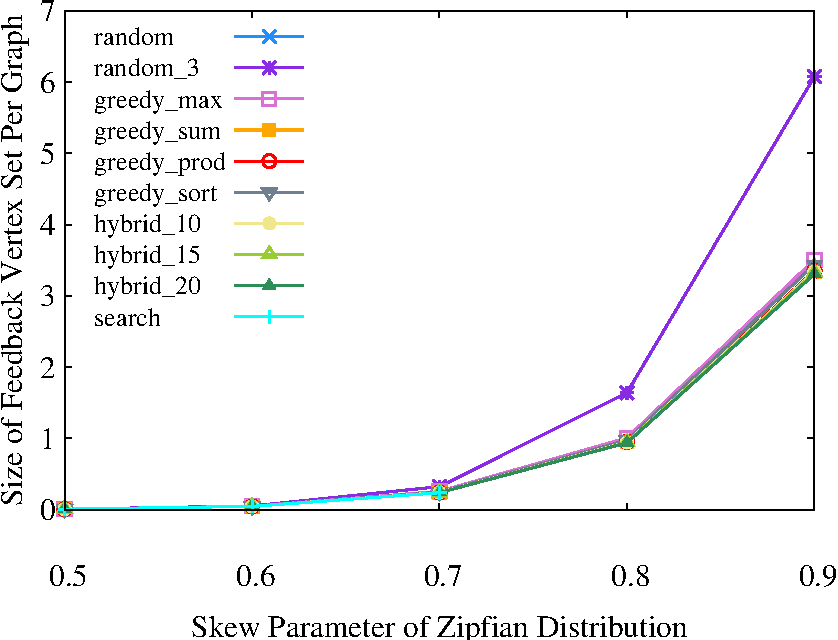
\includegraphics[width=.4\textwidth]{./exp_fig/fvs/fvs}
        %\vspace{-2em}
        \caption{Size of FVS per graph}
        \label{fig:fvs:fvs}
%    \end{minipage}
\end{figure}

\begin{figure}[t]
%    \begin{minipage}[b]{0.48\linewidth}
        \centering
        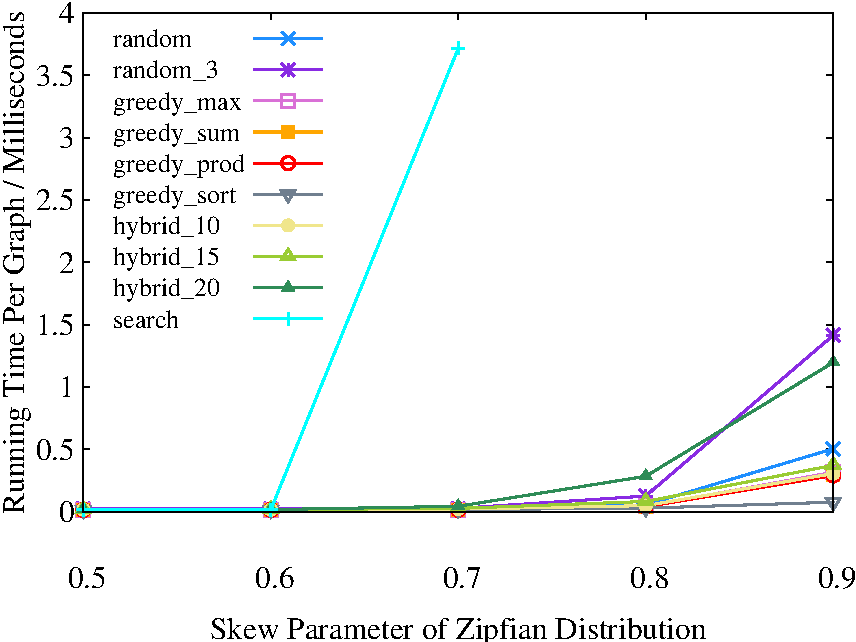
\includegraphics[width=.4\textwidth]{./exp_fig/fvs/latency}
        %\vspace{-2em}
        \caption{Running time of finding FVS}
        \label{fig:fvs:latency}
%    \end{minipage}
\end{figure}


\begin{figure*}[t]
	\centering
    \begin{minipage}[b]{0.31\linewidth}
        \centering
        \includegraphics[width=\textwidth]{./exp_fig/greedy/tps}
        %\vspace{-2em}
        \caption{Throughput with different greedy algorithms}
        \label{fig:greedy:tps}
    \end{minipage}
    \begin{minipage}[b]{0.31\linewidth}
	\centering
	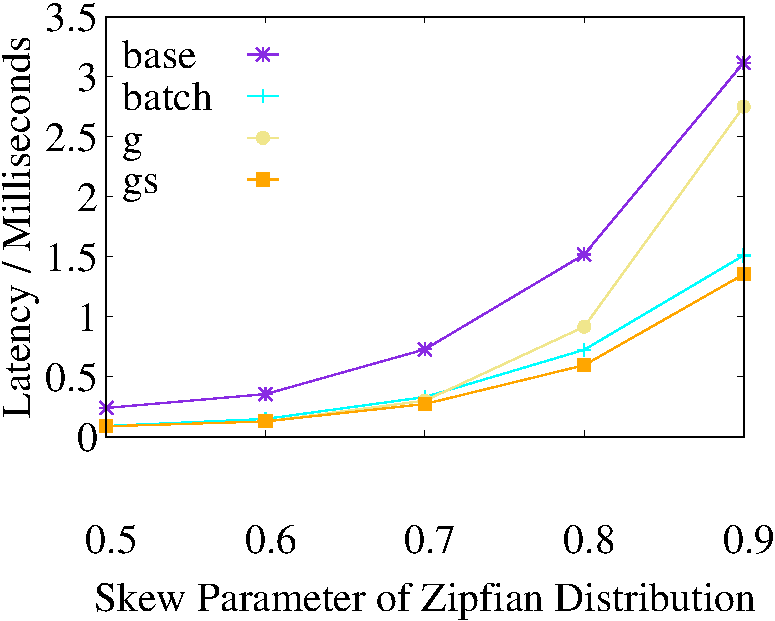
\includegraphics[width=\textwidth]{./exp_fig/greedy/latency}
	%\vspace{-2em}
	\caption{Average latency with different greedy algorithms}
	\label{fig:greedy:latency}
	\end{minipage}
    \begin{minipage}[b]{0.31\linewidth}
        \centering
        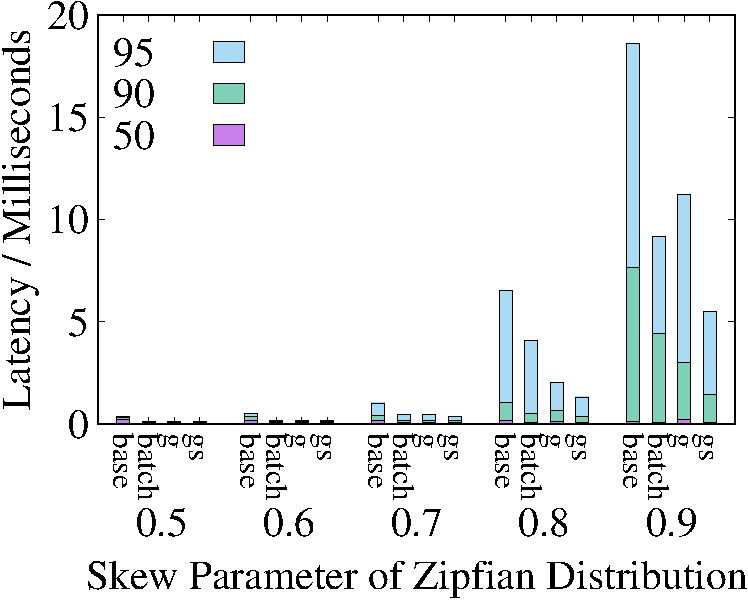
\includegraphics[width=\textwidth]{./exp_fig/greedy/percent95_latency}
     %   \vspace{-2em}
        \caption{Percentile latency with different greedy algorithms}
        \label{fig:greedy:p95}
    \end{minipage}
\end{figure*}


\begin{figure*}[t]
	\centering
	\begin{minipage}[b]{0.31\linewidth}
	\centering
	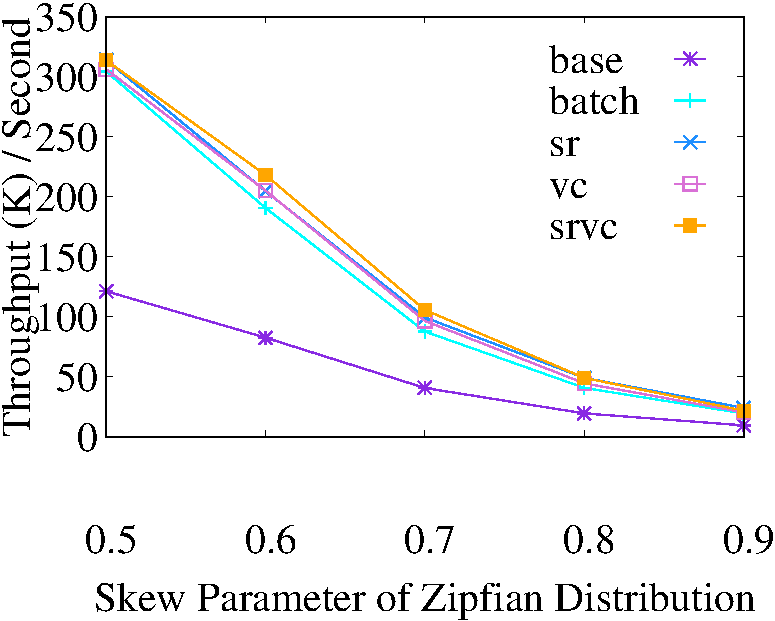
\includegraphics[width=\textwidth]{./exp_fig/basic/tps}
	%vspace{-2em}
	\caption{Throughput under workloads of Zipfian distribution}
	\label{fig:basic:tps}
	\end{minipage}    
    \begin{minipage}[b]{0.31\linewidth}
    	\centering
    	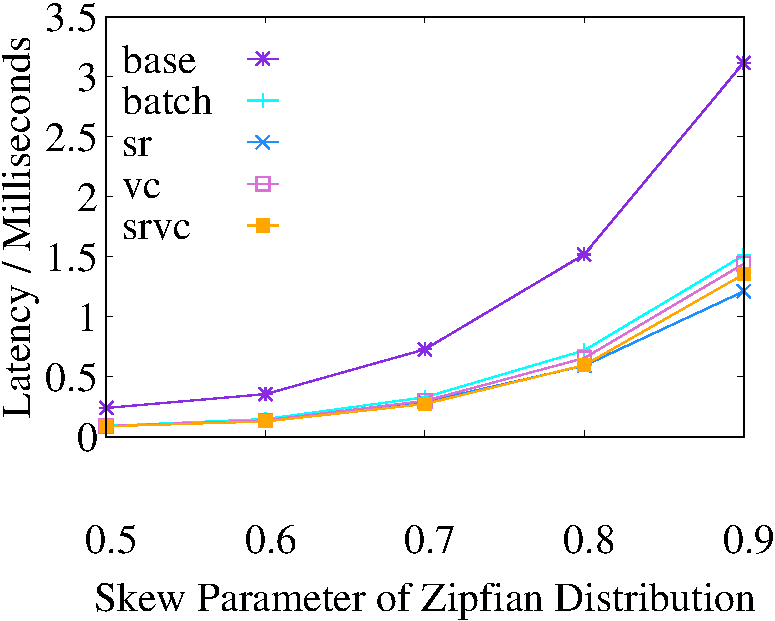
\includegraphics[width=\textwidth]{./exp_fig/basic/latency}
    %	\vspace{-2em}
    	\caption{Average latency under workloads of Zipfian distribution}
    	\label{fig:basic:latency}
    \end{minipage}
    \begin{minipage}[b]{0.31\linewidth}
    	\centering
    	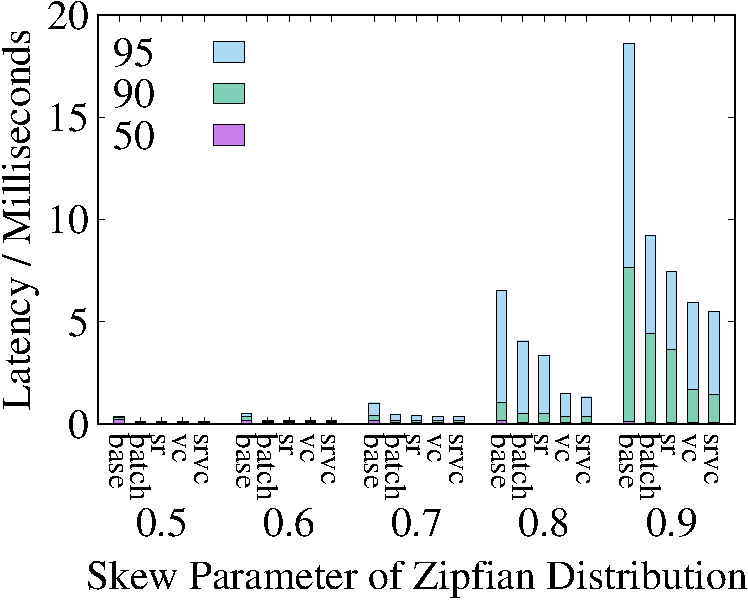
\includegraphics[width=\textwidth]{./exp_fig/basic/percent95_latency}
    %	\vspace{-2em}
    	\caption{Percentile latency under workloads of Zipfian distribution}
    	\label{fig:basic:p95}
    \end{minipage}
\end{figure*}


\begin{figure*}[t]
	\centering
	%	\begin{minipage}[b]{0.31\linewidth}
	%	\centering
	%	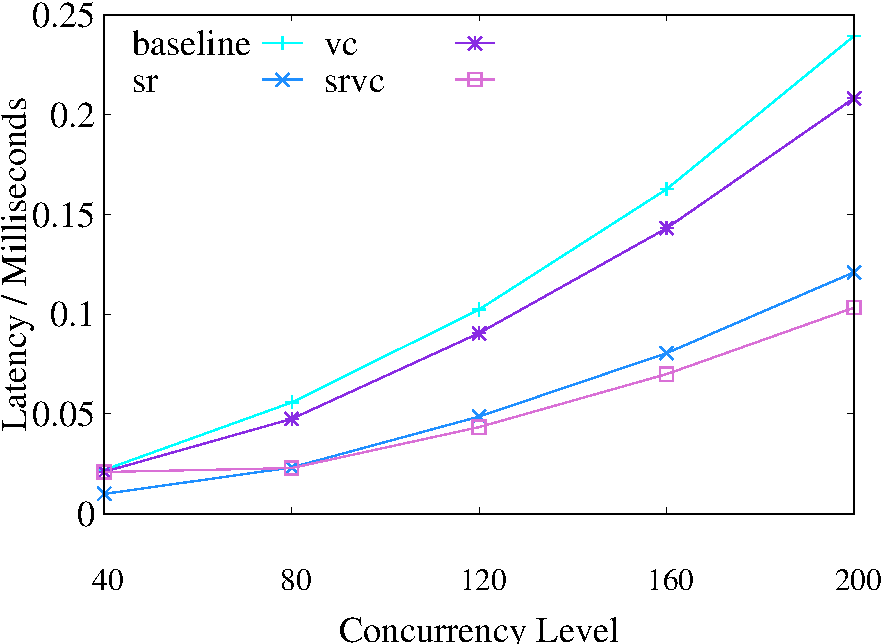
\includegraphics[width=\textwidth]{{{./exp_fig/load/Z0.8_latency}}}
	%	\vspace{-2em}
	%	\caption{Average latency with micro benchmark (skew factor 0.8)}
	%	\label{fig:load_z0.8:latency}
	%\end{minipage}
	\begin{minipage}[b]{0.31\linewidth}
		\centering
		\includegraphics[width=\textwidth]{{{./exp_fig/small_bank/tps}}}
		%	\vspace{-2em}
		\caption{Throughput with Small Bank benchmark}
		\label{fig:small_bank:tps}
	\end{minipage}
	\begin{minipage}[b]{0.31\linewidth}
		\centering
		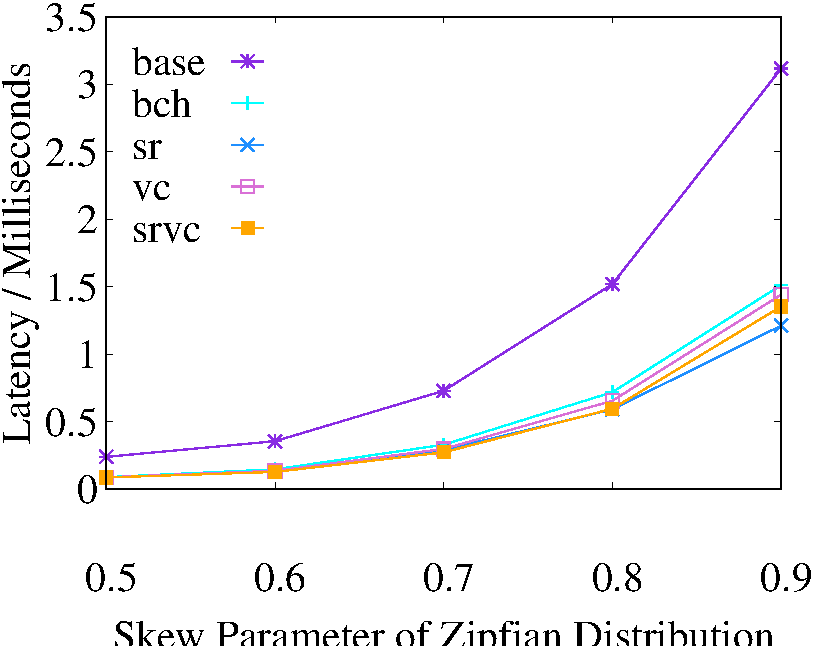
\includegraphics[width=\textwidth]{{{./exp_fig/small_bank/latency}}}
		%	\vspace{-2em}
		\caption{Average latency with Small Bank benchmark}
		\label{fig:small_bank:latency}
	\end{minipage}
	\begin{minipage}[b]{0.31\linewidth}
		\centering
		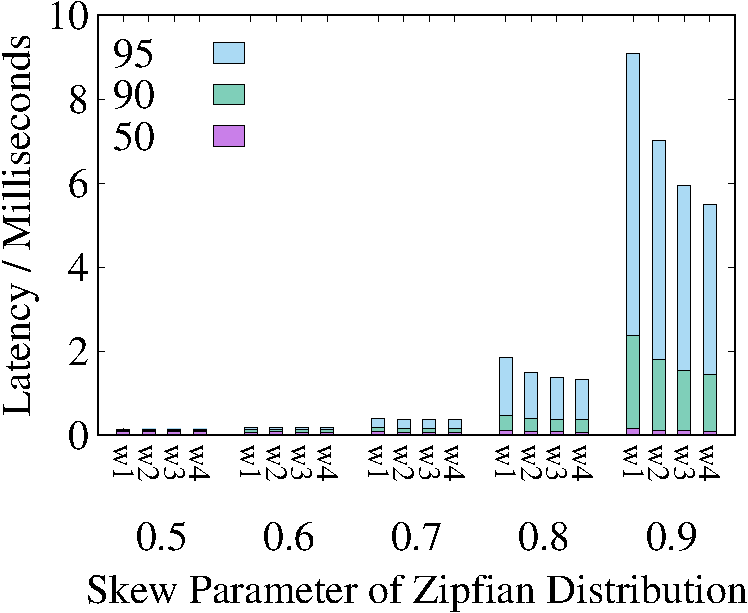
\includegraphics[width=\textwidth]{{{./exp_fig/small_bank/percent95_latency}}}
		%	\vspace{-2em}
		\caption{Percentile latency with Small Bank benchmark}
		\label{fig:small_bank:p95}
	\end{minipage}
	%	 \begin{minipage}[b]{0.31\linewidth}
	%	\centering
	%	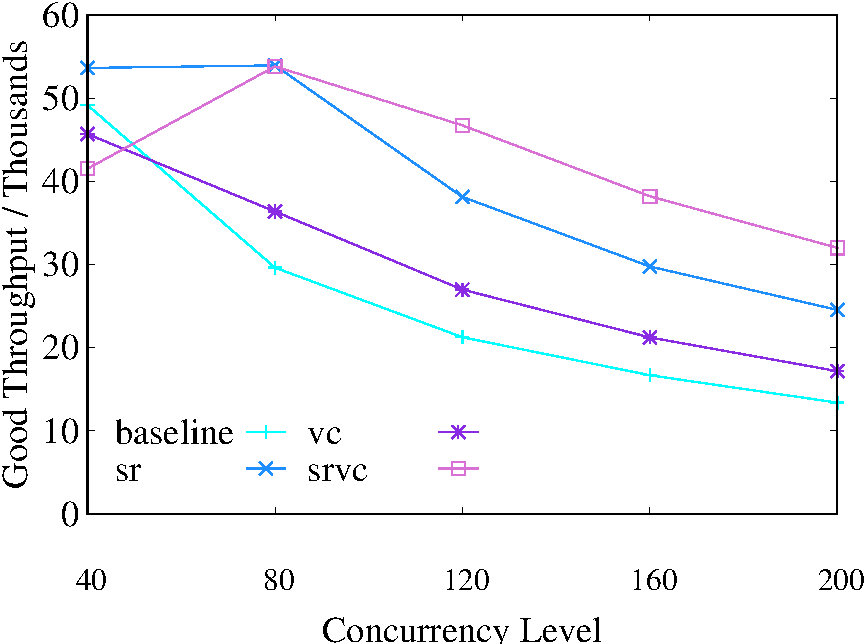
\includegraphics[width=\textwidth]{{{./exp_fig/small_bank/Z0.9_tps}}}
	%	\vspace{-2em}
	%	\caption{Throughput with Small Bank benchmark (skew factor 0.9)}
	%	\label{fig:small_bank_z0.9:tps}
	%	\end{minipage}
	%	\begin{minipage}[b]{0.31\linewidth}
	%	\centering
	%	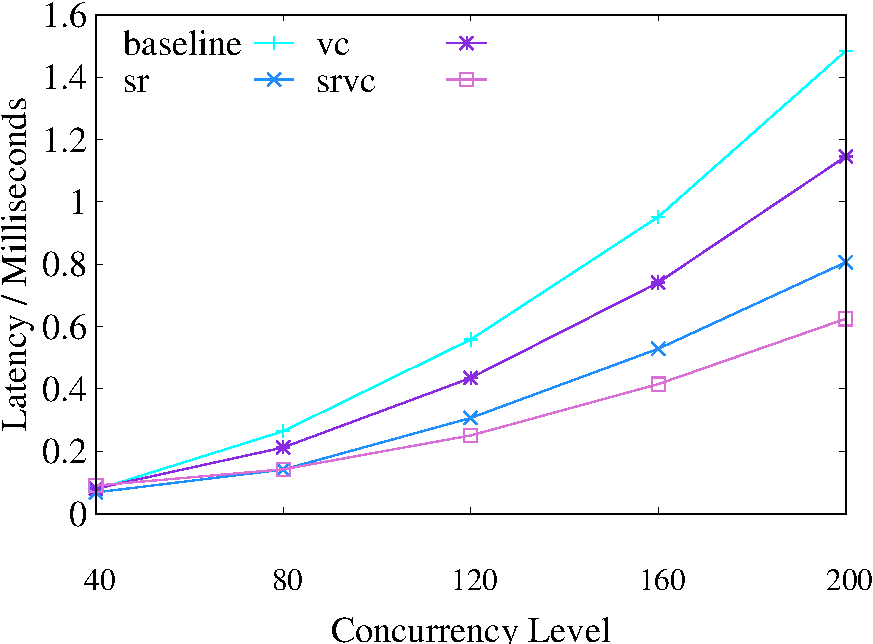
\includegraphics[width=\textwidth]{{{./exp_fig/small_bank/Z0.9_latency}}}
	%	\vspace{-2em}
	%	\caption{Average latency with Small Bank benchmark (skew factor 0.9)}
	%	\label{fig:small_bank_z0.9:latency}
	%	\end{minipage}
	%    \vspace{-1em}
\end{figure*}

\begin{figure*}[t]
	\centering
	\begin{minipage}[b]{0.31\linewidth}
	\centering
	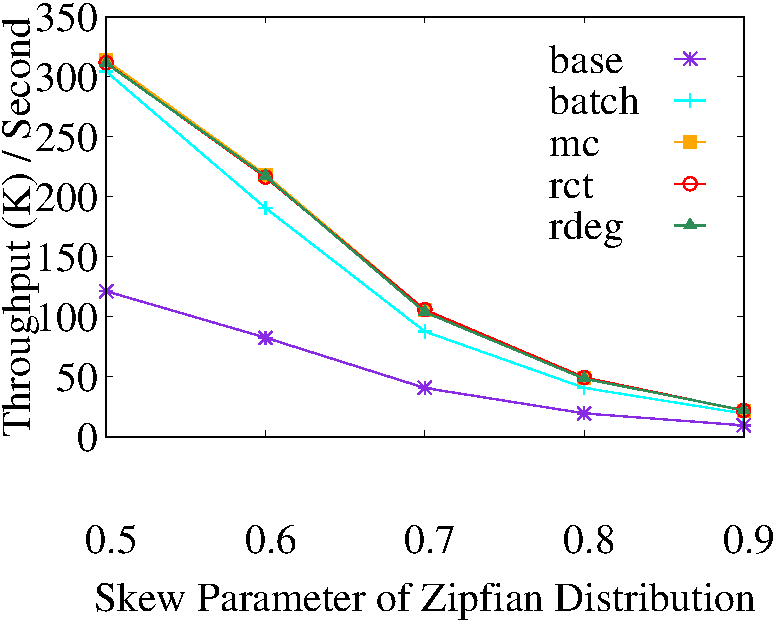
\includegraphics[width=\textwidth]{./exp_fig/restart/tps}
%	\vspace{-2em}
	\caption{Throughput with tail latency optimized policies}
	\label{fig:restart:tps}
	\end{minipage}
	\begin{minipage}[b]{0.31\linewidth}
		\centering
		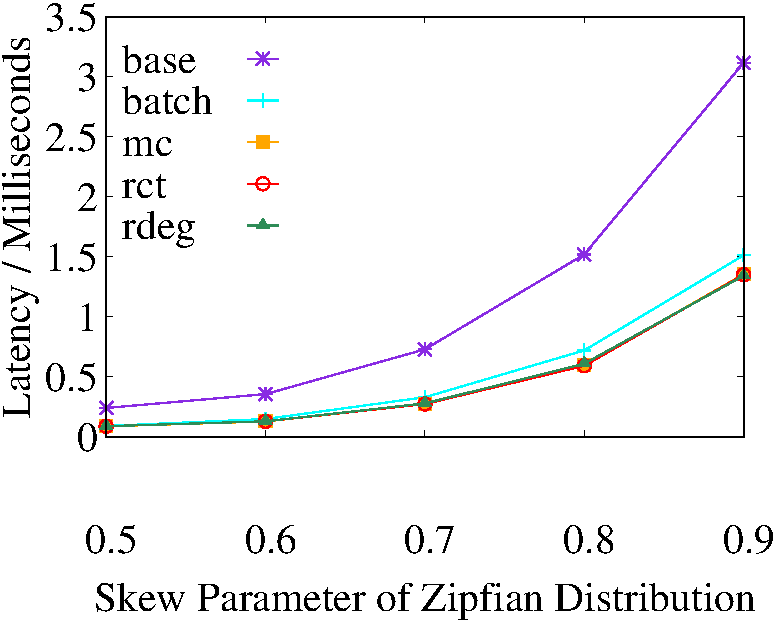
\includegraphics[width=\textwidth]{./exp_fig/restart/latency}
%		\vspace{-2em}
		\caption{Average latency with tail latency optimized policies}
		\label{fig:restart:latency}
	\end{minipage}
	\begin{minipage}[b]{0.31\linewidth}
	\centering
	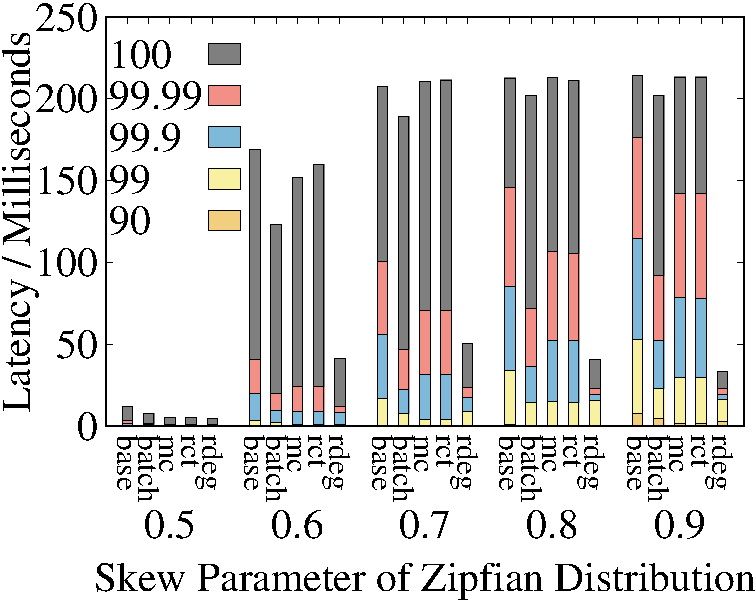
\includegraphics[width=\textwidth]{./exp_fig/restart/percent100_latency}
%	\vspace{-2em}
	\caption{Percentile latency with tail latency optimized policies}
	\label{fig:restart:p100}
	\end{minipage}
\end{figure*}


%\begin{figure*}[t]
%    \centering
%    \begin{minipage}[b]{0.31\linewidth}
%	\centering
%	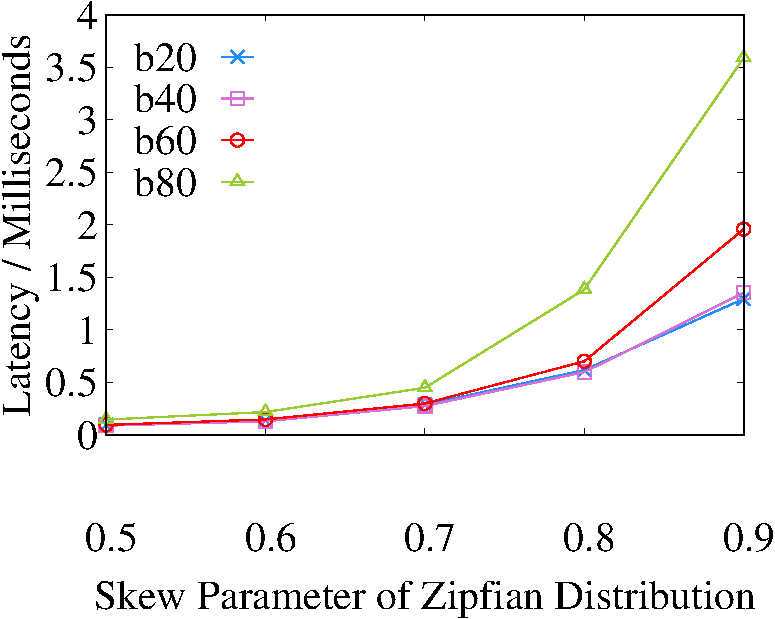
\includegraphics[width=\textwidth]{./exp_fig/bsize/latency}
%	\vspace{-2em}
%	\caption{Average latency with various batch sizes}
%	\label{fig:bsize:latency}
%	\end{minipage}
 %   \begin{minipage}[b]{0.31\linewidth}
%	\centering
%	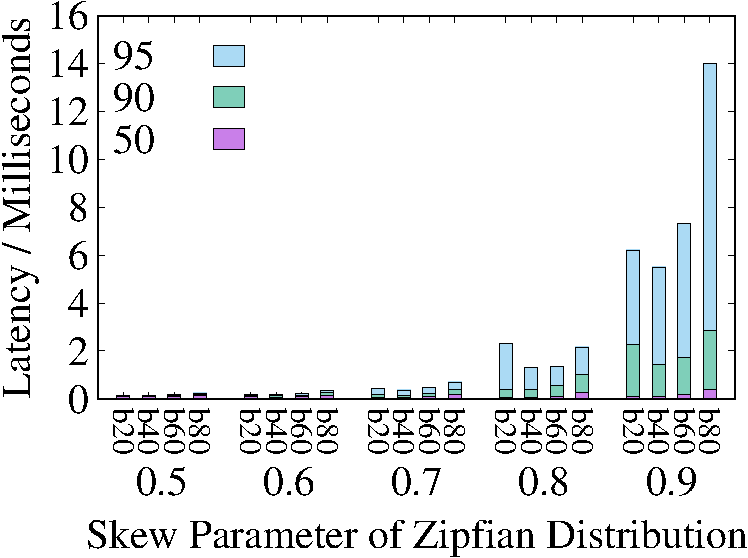
\includegraphics[width=\textwidth]{./exp_fig/bsize/percent95_latency}
%	\vspace{-2em}
%	\caption{Percentile latency with various batch sizes}
%	\label{fig:bsize:p95}
%	\end{minipage}

%    \vspace{-1em}
%\end{figure*}

%\begin{figure*}[t]
%    \centering
    
%   \begin{minipage}[b]{0.31\linewidth}
%	\centering
%	\includegraphics[width=\textwidth]{{{./exp_fig/load/Z0.7_tps}}}
%	\vspace{-2em}
%	\caption{Throughput with fixed workload (skew factor 0.7)}
%	\label{fig:load_z0.7:tps}
%	\end{minipage}
%    \vspace{-1em}
%\end{figure*}



%\begin{figure*}[t]
%    \centering
%    \begin{minipage}[b]{0.31\linewidth}
%	\centering
%	\includegraphics[width=\textwidth]{{{./exp_fig/load/Z0.7_latency}}}
%	\vspace{-2em}
%	\caption{Average latency with micro benchmark (skew factor 0.7)}
%	\label{fig:load_z0.7:latency}
%	\end{minipage}
%\end{figure*}

%\begin{figure*}[t]
%    \centering
%    \begin{minipage}[b]{0.31\linewidth}
%	\centering
%	\includegraphics[width=\textwidth]{{{./exp_fig/small_bank/Z0.7_tps}}}
%	\vspace{-2em}
%	\caption{Throughput with Small Bank benchmark (skew factor 0.7)}
%	\label{fig:small_bank_z0.7:tps}
%	\end{minipage}
%   \begin{minipage}[b]{0.31\linewidth}
%       \centering
%        \includegraphics[width=\textwidth]{{{./exp_fig/small_bank/Z0.7_latency}}}
%        \vspace{-2em}
%        \caption{Average latency with Small Bank benchmark (skew factor 0.7)}
%        \label{fig:small_bank_z0.7:latency}
%    \end{minipage}
%	 \begin{minipage}[b]{0.31\linewidth}
%	\centering
%	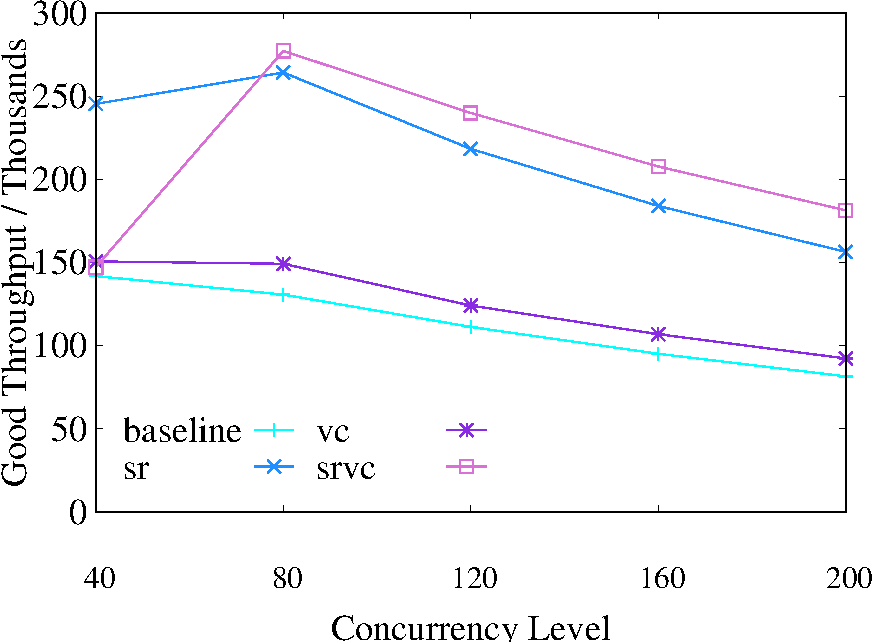
\includegraphics[width=\textwidth]{{{./exp_fig/small_bank/Z0.8_tps}}}
%	\vspace{-2em}
%	\caption{Throughput with Small Bank benchmark (skew factor 0.8)}
%	\label{fig:small_bank_z0.8:tps}
%	\end{minipage}
%    \vspace{-1em}
%\end{figure*}


\begin{figure*}[t]
	\centering
	\begin{minipage}[b]{0.31\linewidth}
		\centering
		\includegraphics[width=\textwidth]{./exp_fig/oltp_kernel/pdf/{tps_r0.5_z0.99}.pdf}
		%		\vspace{-2em}
		\caption{Throughput of YCSB with skew factor 0.99}
		\label{fig:oltp_kernel:tps_z0.99}
	\end{minipage}
	\begin{minipage}[b]{0.31\linewidth}
		\centering
		\includegraphics[width=\textwidth]{./exp_fig/oltp_kernel/pdf/{tps_r0.5_t28}.pdf}
		%	\vspace{-2em}
		\caption{Throughput of YCSB with 28 threads}
		\label{fig:oltp_kernel:tps_t28}
	\end{minipage}
	\begin{minipage}[b]{0.31\linewidth}
		\centering
		\includegraphics[width=\textwidth]{./exp_fig/oltp_kernel/pdf/{latency_r0.5_t28}.pdf}
		%	\vspace{-2em}
		\caption{Percentile latency of YCSB with 28 threads}
		\label{fig:oltp_kernel:latency}
	\end{minipage}
\end{figure*}


\begin{figure*}[t]
	\centering
	%	\begin{minipage}[b]{0.31\linewidth}
	%	\centering
	%	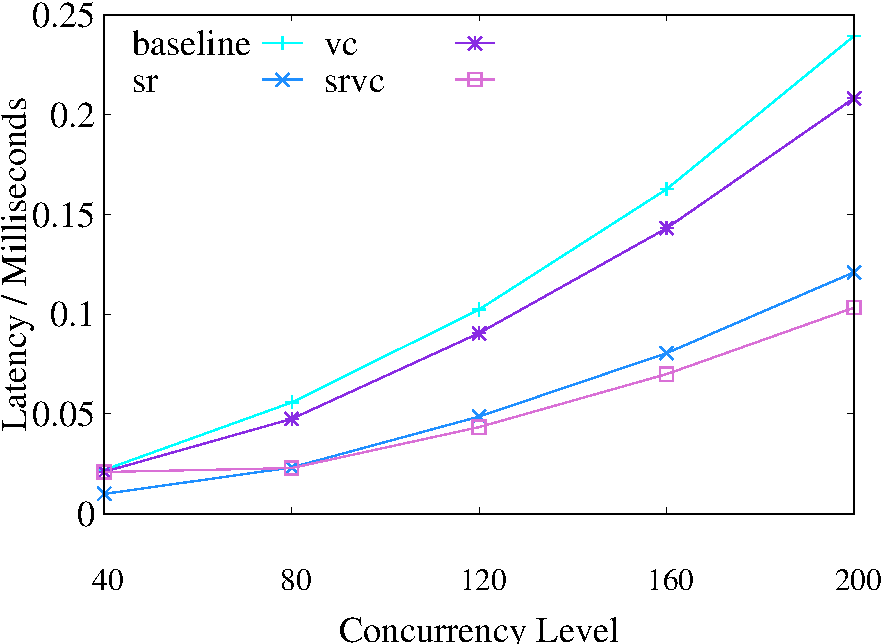
\includegraphics[width=\textwidth]{{{./exp_fig/load/Z0.8_latency}}}
	%	\vspace{-2em}
	%	\caption{Average latency with micro benchmark (skew factor 0.8)}
	%	\label{fig:load_z0.8:latency}
	%\end{minipage}
	\begin{minipage}[b]{0.31\linewidth}
		\centering
		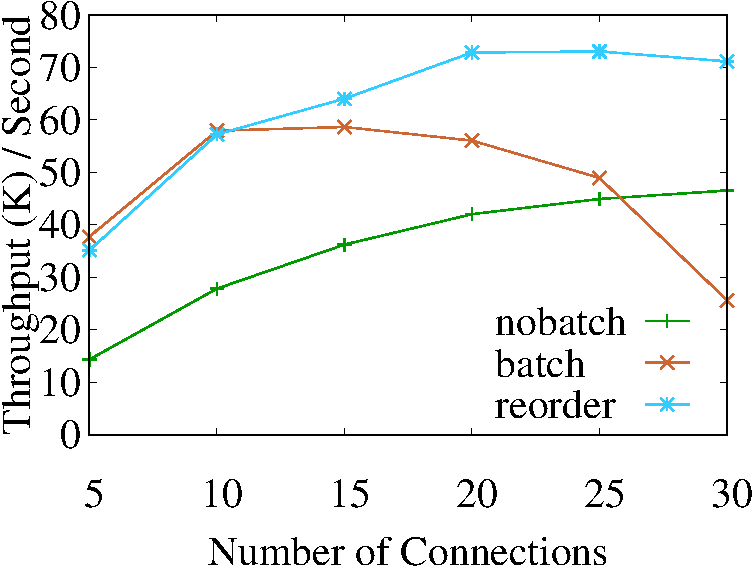
\includegraphics[width=\textwidth]{./exp_fig/hekaton/pdf/hekaton_tps}
		%		\vspace{-2em}
		\caption{Throughput of DBMS-X with SmallBank benchmark}
		\label{fig:hekaton:tps}
	\end{minipage}
	\begin{minipage}[b]{0.31\linewidth}
		\centering
		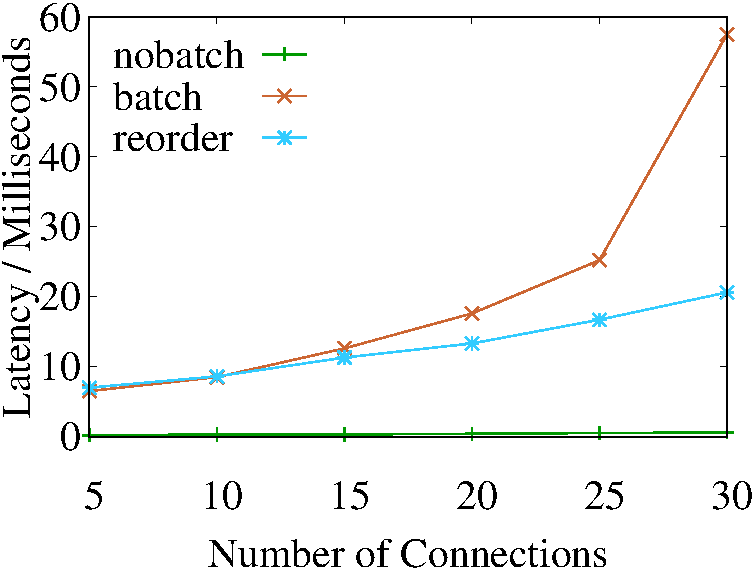
\includegraphics[width=\textwidth]{./exp_fig/hekaton/pdf/hekaton_latency}
		%	\vspace{-2em}
		\caption{Average latency of DBMS-X with SmallBank benchmark}
		\label{fig:hekaton:latency}
	\end{minipage}
	\begin{minipage}[b]{0.31\linewidth}
		\centering
		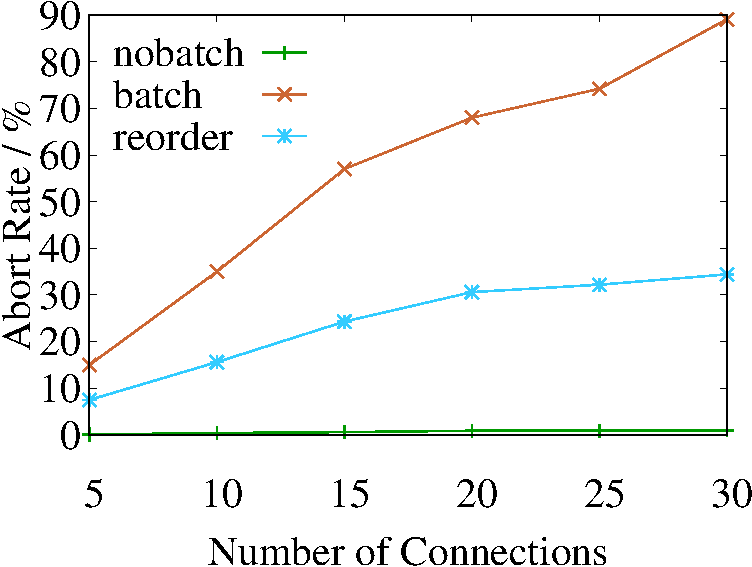
\includegraphics[width=\textwidth]{./exp_fig/hekaton/pdf/hekaton_abort}
		%	\vspace{-2em}
		\caption{Abort rate of DBMS-X with SmallBank benchmark}
		\label{fig:hekaton:abort}
	\end{minipage}
	%	\begin{minipage}[b]{0.31\linewidth}
	%	\centering
	%	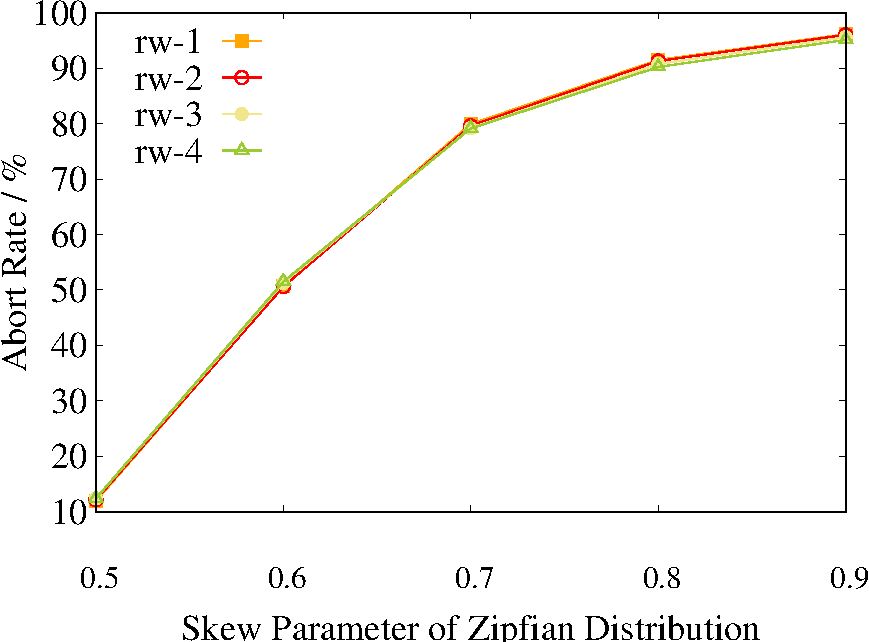
\includegraphics[width=\textwidth]{{{./exp_fig/compare/abort}}}
	%	\vspace{-2em}
	%	\caption{Abort rate with micro benchmark}
	%	\label{fig:compare:abort}
	%	\end{minipage}
	%	 \begin{minipage}[b]{0.31\linewidth}
	%	\centering
	%	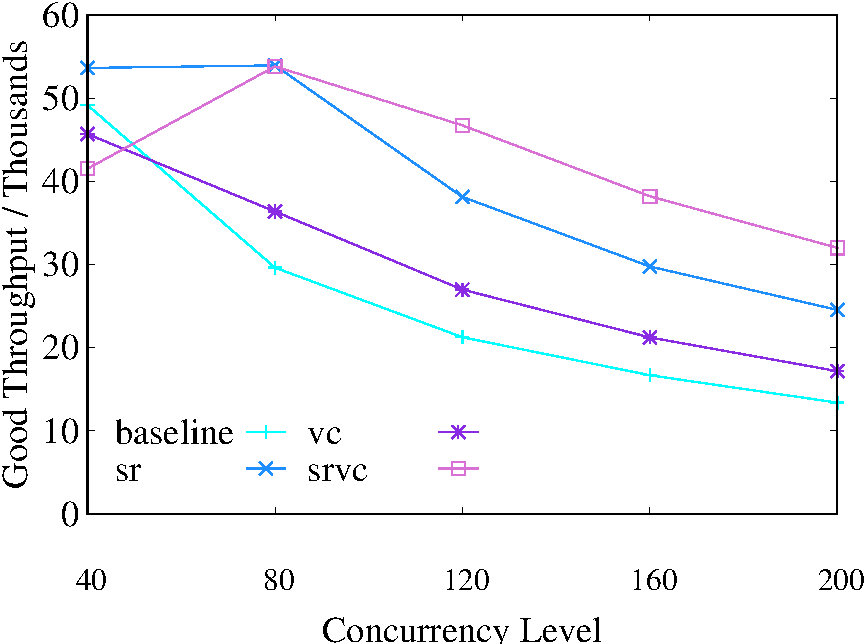
\includegraphics[width=\textwidth]{{{./exp_fig/small_bank/Z0.9_tps}}}
	%	\vspace{-2em}
	%	\caption{Throughput with Small Bank benchmark (skew factor 0.9)}
	%	\label{fig:small_bank_z0.9:tps}
	%	\end{minipage}
	%	\begin{minipage}[b]{0.31\linewidth}
	%	\centering
	%	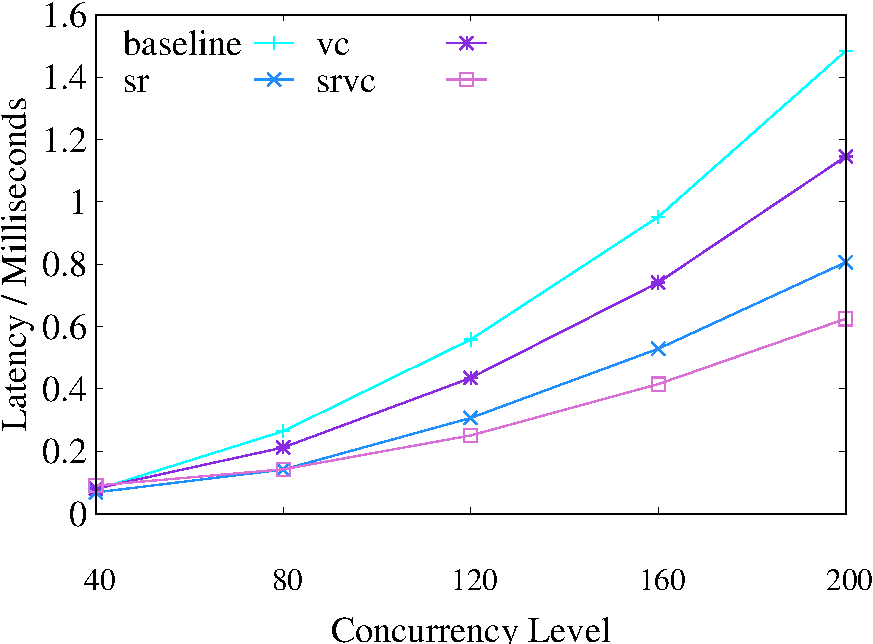
\includegraphics[width=\textwidth]{{{./exp_fig/small_bank/Z0.9_latency}}}
	%	\vspace{-2em}
	%	\caption{Average latency with Small Bank benchmark (skew factor 0.9)}
	%	\label{fig:small_bank_z0.9:latency}
	%	\end{minipage}
	%    \vspace{-1em}
\end{figure*}

% *******************
% * Experiments
% *******************
\subsection{Validator Reordering Algorithms}
\label{sec:exp_algorithms}
We first investigate the performance of the feedback vertex set algorithms from Section~\ref{subsec:validator_reordering:algorithm} 
%with a comparison of the raw performance of the algorithms, i.e., 
for their accuracy and running time. We run the algorithms on graphs constructed as described in Section~\ref{sec:valbatching}, using our micro benchmarks. 
%\eat{We first test the algorithms offline on the dependency graphs constructed at validator when running the system. Each dependency graph is constructed from a batch of transactions at validator, excluding non-viable transactions, i.e., we only use transactions that don't have inter-batch conflicts. We compare the averages of the size of the feedback vertex set and the running time per dependency graph.}
We test the SCC-based greedy algorithm with the \texttt{max-degree} ($greedy\_max$), \texttt{sum-degree} ($greedy\_sum$) and \texttt{prod-degree} policies ($greedy\_prod$). We also test the sort-based greedy algorithm $greedy\_sort$ (using the \texttt{prod-degree} policy for sorting and multi factor 2), as well as the hybrid algorithm $hybrid\_m$. The hybrid algorithm uses $greedy\_prod$ as a subroutine when the size of the SCC is larger than $m$, and switches to the brute force search otherwise. By increasing the threshold, we can progressively approximate the optimal solution. 
We test these algorithms against several baselines: $search$ is an accurate,
brute force search algorithm; $random$ is the SCC-based greedy algorithm which
removes a vertex at random from each SCC to break the cycle. For each graph constructed from a batch of transactions,
$random\_3$ runs $random$ 3 times and returns the smallest FVS, mitigating the
effect of bad random choices.

Figure~\ref{fig:fvs:fvs} shows the average size of the feedback vertex set found by each algorithm. The brute force search algorithm is so slow that it cannot produce results once the skew factor increases beyond $0.7$ as the graphs become denser.
The $random$ baseline computes a FVS whose size is almost twice as large as the greedy and the hybrid algorithms. Running the random algorithm multiple times produces similar results. This confirms the theoretical results which show that finding a good FVS is hard. The greedy algorithms, on the other hand, produce very accurate results. The average size of the FVS is almost identical to that of the brute force search when the skew factor is no larger than $0.7$, and is very close to the best hybrid algorithm ($hybrid\_20$, i.e., one that uses the brute force search when the size of the SCC is no larger than 20). Among the greedy algorithms, $greedy\_prod$ is consistently the best, although the difference is small.

Figure~\ref{fig:fvs:latency} shows the running time of the algorithms. The running time of the hybrid algorithm depends on the threshold for switching to brute force search. Thus, $hybrid\_20$ and $hybrid\_15$ have a longer running time than other algorithms, while the running time of $hybrid\_10$ is comparable to the SCC-based algorithms. Each of the SCC-based algorithms ($greedy\_max$, $greedy\_sum$, $greedy\_prod$, $random$) has a similar running time. The random algorithm takes slightly longer than the greedy algorithms because it removes more nodes and thus requires more iterations to find FVS. The running time of $random\_3$ is three times that of $random$, since it runs the random algorithm three times. The sort-based greedy algorithm ($greedy\_sort$), while slightly less accurate than the SCC-based greedy algorithms, reduces the running time of these algorithms by 74\%. 

We compare the end-to-end performance of the best SCC-based algorithm ($greedy\_prod$) with the sort-based greedy algorithm. Figure~\ref{fig:greedy:tps} and~\ref{fig:greedy:latency} show the throughput and the average latency of the system with $greedy\_prod$ ($g$) and $greedy\_sort$ ($gs$). In both cases, storage batching is enabled. The $base$ line shows the throughput with both storage and validator batching disabled. 
The two greedy algorithms have similar throughput when the skew is very low. However, $greedy\_prod$ degrades significantly with increasing data skew. This is because while $greedy\_prod$ is slightly more accurate, it takes much longer to run. This increases transaction latency and leads to more conflicts, especially when the data contention is high. $greedy\_sort$ consistently gives the highest throughput over all the workloads for its high accuracy and low running time. 
Figure~\ref{fig:greedy:p95} shows transaction latency by percentile, i.e., the latency threshold for up to 95\% of the transactions. The tail latency of $greedy\_sort$ is much lower than that of the other two, which is consistent with the throughput data.

\eat{In summary, the sort-based greedy algorithm is much faster than the ``smarter'' algorithms and only slightly worse in terms of accuracy, resulting in the best end-to-end system performance. For this reason, all subsequent experiments use the sort-based greedy algorithm with a \texttt{prod-degree} policy unless otherwise specified.}

%\subsection{Batch Size}
In this experiment, we explore the impact of batch size on system performance. 
Smaller batch sizes should give lower latency but they offer fewer opportunities for reordering, leading to more aborts. 
We configure the system to perform both storage and validator batching with batch sizes from $20$ to $80$.\eat{, using the same batch size at storage and validator. As before, $baseline$ is the system with both types of batching turned off. }
Figure~\ref{fig:bsize:tps} and~\ref{fig:bsize:latency} shows the throughput and average latency with different batch sizes as data skew increases. The throughput first rises as we increase the size of the batch, and then degrades when the batch becomes too large. Batch size 40 gives the best throughput and the latency. The percentile latency displays a similar pattern, as shown in Figure~\ref{fig:bsize:p95}.

 \eat{Again the best batch size is 40. However, using batching always gives higher throughput and a better latency profile than the baseline.Given the above results, a batch size of 40 appears optimal for our configuration; we use this batch size in the remainder of our experiments. }

\subsection{Storage and Validator Batching}
\label{subsec:experiment:batching}

Next, we perform a detailed analysis on the effects of storage and validator batching. We configure the system in several different modes: no batching ($base$), batching without reordering (\changed{$batch$}), storage only batching with reordering ($sr$), validator only batching with reordering
%\eat{with the \texttt{prod-degree} policy that maximizes the number of commits }
($vc$), and both storage and validator batching with reordering ($srvc$).


\eat{As explained in Section~\ref{sec:overview}, batching and reordering affect the abort rate by reducing inter-batch and intra-batch aborts. The number of inter-batch aborts is affected by system-wide transaction latency, the freshness of the transactions' reads, and their access patterns. Validator reordering reduces the number of intra-batch aborts; however, storage reordering can increase the number of such aborts because it reduces inter-batch aborts (and thus more viable transactions end up in validator batches rather than aborting due to inter-batch conflicts). The overall throughput of the system is affected by both the transaction latency and the abort rate. }%end of \eat


Figures~\ref{fig:basic:tps},~\ref{fig:basic:latency}, and~\ref{fig:basic:p95} show the throughput, the average and percentile latency of different system modes under various data skews. Using batching with reordering at the storage and/or validator consistently improves throughput by up to 2.7x. \cut{Reordering ($vrsr$) on top of batching (\changed{$batch$}) improves the throughput to up to $1.3\times$.} Moreover, validator reordering significantly reduces the average and tail latency by up to $67\%$ and $82\%$ respectively, compared with the baseline ($base$).\cut{, and by up to 25\% and 70\% as compared to \changed{$batch$}.}

%\eat{When batching is enabled ($sr$ and $srvc$), the throughput is 2.1x-2.4x that of the baseline ($baseline$). In addition, using validator batching always gives a better latency profile (Figure~\ref{fig:basic:p95}).}
%\eat{When the data contention is very low, the abort rate is low. Thus, the storage-batching-only mode ($sr$) gives similar throughput compared with $srvc$.  As the data skew increases, so does the number of intra-batch conflicts and aborts; the overhead of validator batching starts to pay off. In a medium-contention setting, using both validator and storage batching ($srvc$) gives the best throughput.}
When the data contention is extremely high (i.e., skew factor 0.9), the number of intra-batch conflicts
that cannot be resolved by validator reordering increases. Validator reordering
is slower due to denser graphs, while bringing less benefit. Thus, the best throughput in this case is achieved by using storage only batching with reordering ($sr$). 

\eat{We conducted additional experiments to evaluate the performance with a fixed workload and varying load. Figure~\ref{fig:load_z0.7:tps} shows the throughput of the system with skew factor 0.7. The configuration that enables both storage and validator batching with reordering consistently outperforms the others. The throughput increases by up to 2.5x, and the average latency is reduced by up to 63\% as compared to $base$. More figures on additional metrics and parameters are omitted due space limits.}

\eat{
To summarize, it is always beneficial to enable storage batching since this technique reduces inter-batch aborts at a minimal cost. While validator batching consistently gives a percentile latency, it is most effective in mid-contention settings, when the reduction of intra-batch conflicts that it brings is sufficient to justify its cost. }

We further evaluate batching and reordering on the Small Bank benchmark~\cite{alomari2008icde}. The Small Bank benchmark contains transactions with a realistic and diverse
combination of read and write conflicts: compute the balance of a customer's checking and savings
accounts, deposit money to a checking account, transfer money from a checking
account to a savings account, move funds from one customer to another, and withdraw money from a customer's account. We use a Zipfian distribution to simulate skewed data accesses. We populate the database with 100K customers, including 100K checking and 100K savings accounts.

Figure~\ref{fig:small_bank:tps},~\ref{fig:small_bank:latency},~\ref{fig:small_bank:p95} show the throughput, the average and percentile latency of transactions. The result is very similar to that on our micro benchmark.

\cut{
Figure~\ref{fig:small_bank:tps},~\ref{fig:small_bank:latency},~\ref{fig:small_bank:p95} show the throughput, the average and percentile latency of transactions.\cut{ Overall, batching and reordering improved the throughput by up to $3.1\times$, reduced average latency by up to $68\%$, and tail latency by up to $62\%$.} The benefits of batching and reordering are similar to these on our micro benchmark.\cut{, storage and validator reordering can always improve the throughput and reduce the latency on top of batching. confirming our findings in Section~\ref{subsec:experiment:batching}.}}


\subsection{Small Bank Benchmark}
\label{subsec:experiment:end2end}
\eat{In our final experiment, we explore the end-to-end performance of batching in a realistic setting where batch size is fixed. We use two workloads: a micro benchmark and the Small Bank benchmark~\cite{alomari2008icde}. In our micro benchmark,  we generate the transactions as described in Section~\ref{subsec:experiment:implementation}. \eat{We introduce skewed accesses to the data where each object is drawn from Zipfian distribution.} }

\eat{In this experiment, we explore the end-to-end performance of batching in a realistic setting. We choose the same Small Bank benchmark as in Section~\ref{subsec:experiment:compare}.}

The Small Bank benchmark~\cite{alomari2008icde} contains transactions with a realistic and diverse
combination of read and write conflicts. The transactions come from the
financial domain: compute the balance of a customer's checking and savings
accounts, deposit money to a checking account, transfer money from a checking
account to a savings account, move funds from one customer to another, and withdraw money from a customer's account. We use a Zipfian distribution to simulate skewed data accesses. We populate the database with 100K customers, i.e., 100K checking and 100K savings accounts.

\eat{We use a batch size of 10 transactions and we vary the system concurrency level from 20 to 140 transactions. We simulate high data contention by introducing Zipfian skew factor (0.5-0.9 for the micro benchmark and 0.7-0.9 for the Small Bank benchmark, which has shorter transactions).
\eat{, i.e., the limit of active transactions in the system}}%eat
% Overall performance.
\eat{Overall, in the micro benchmark, batching has improved the throughput up to 2.4x, while reduced up to 58\% of the average latency. In Small Bank benchmark, batching has improved the throughput up to 3.1x, while reduced up to 68\% of the average latency.}%eat

Figure~\ref{fig:small_bank:tps},~\ref{fig:small_bank:latency},~\ref{fig:small_bank:p95} show the throughput, the average latency, and the percentile latency of transactions. Overall, batching and reordering improved the throughput up to 3.1x, reduced average latency by up to 68\%, and tail latency by up to 62\%. Storage and validator reordering can always improve the throughput and reduce the latency on top of batching, confirming our findings in Section~\ref{subsec:experiment:batching}.

\eat{On the micro benchmark, Figure~\ref{fig:load_z0.7:tps} shows the throughput with skew factor 0.7. Overall, batching has improved the throughput 
Using batching doubles the throughput as compared to the baseline, both for a given load and when considering the peak throughput over different loads. When the load is moderate, storage batching by itself performs best. As the load increases and the transactions become more conflict-prone, the benefit of validator batching outweighs its cost. }

\eat{Figure~\ref{fig:load_z0.7:latency} shows the average transaction latency with skew factor 0.7. Both storage and validator batching reduce the latency as compared to the baseline. Validator batching gives the lowest latency when the data is extremely skewed. In addition, validator batching always reduces latency regardless of whether storage batching is enabled, again confirming our findings in Section~\ref{subsec:experiment:batching}. The performance impacts of batching are similar to those on the micro benchmark. 

The experiments with additional parameters show similar performance impact with batching. We omit the figures due to the space limit.}%eat
 % include load and small bank experiments.

\subsection{More Policies for Validator Reordering: Reducing Tail Latency}

We explore validator reordering with a more complicated policy presented in Section~\ref{subsec:validator_reordering:policy}; specifically, we look at policies that aim to reduce the transaction tail latency.

We explore the possibility of reducing transaction tail latency with latency-specific policies. Our baselines are the \texttt{prod-degree} policy that maximizes the number of commits ($max\hbox{-}c$) as well as the $baseline$ with no batching. 

Our first tail-latency aware policy ($rst\hbox{-}cnt$) favors transactions that have already been aborted and restarted. When choosing a node to include in the feedback vertex set, it chooses the one with the smallest number of restarts, breaking ties using \texttt{prod-degree}.

The second latency-aware policy considers both the number of restarts and a degree-based measurement of a transaction. It computes the weight of a node as the product of in-degree and out-degree over the exponential of the number of restarts with base 2. When choosing a node to include in the feedback vertex set, the nodes are sorted in descending order by their weights. Thus, a node with a high degree product can have its weight reduced if the corresponding transaction has restarted many times.

Figure~\ref{fig:restart:tps} and~\ref{fig:restart:latency} show the transaction throughput and average latency. As expected, the impact of tail-latency aware policies on overall transaction throughput and average latency are negligible as compared towhen we maximize the number of commits ($max\hbox{-}c$).

Figure~\ref{fig:restart:p100} shows the tail latency from 90\% to 100\%, i.e., the latency threshold for from up to 90\% to up to 100\% of the transactions. While maximizing the number of commits, the \texttt{prod-degree} policy can produce worse tail latency than the baseline when the skew factor is high. This is because it is unaware of the restart times of transactions, and it can discriminate against transactions that are inherently hard to commit, e.g., because they access many hot objects. Our first latency-aware policy $rst\hbox{-}cnt$ performs similar as $max-c$.
 
In contrast, while our first latency-aware policy $rst\hbox{-}cnt$ performs similar to $max-c$, the more sophisticated policy $rst\hbox{-}cnt$ consistently performs significantly better than all the others, especially for tail latency from 99.9\% to 100\%.  \eat{, although $rst\hbox{-}deg$ consistently performs slightly better than $rst\hbox{-}cnt$.}

In summary, the latency-aware policies decrease tail latency significantly while maintaining a comparable overall performance to the policy that maximizes the number of commits. Moreover, the latency-ware policy that combines the graph degree and the number of restarts together performs significantly better as compared to the others.

\eat{
\subsubsection{Helping hard transactions commit}

We simulate a heterogeneous workload by including 80\% of normal transactions with 5 reads and 5 writes, and 20\% of ``hard transactions'' with 10 reads and 10 writes. All the data accesses are drawn from the same Zipfian distribution. The larger transactions are more likely to conflict with others and less likely to commit; thus, we assign them higher priorities in the validator reordering. We compare the system performance with unweighted ($srvc$) validator reordering and a weighted ($srvs$) validator reordering policy that privileges the larger transactions. In both cases, storage batching is enabled. As before, the $baseline$ configuration uses no batching.

Figures~\ref{fig:weighted:tps} and~\ref{fig:weighted:p95} show the overall throughput and the percentile latency. Since the ratio of large transactions is small, the overall performance under weighted and unweighted reordering policies is similar.

Figures~\ref{fig:weighted:tps1},~\ref{fig:weighted:abort1}, and~\ref{fig:weighted:p951} show the throughput, the abort rate, and the percentile latency of the larger transactions alone. While the throughput of unweighted and weighted validator reordering is still similar, weighted validator reordering gives a much better transaction profile as far as the abort rate and the percentile latency are concerned.
}
\subsection{Degradation Under Data Contention}
\label{subsec:experiment:compare}

In our final experiment, we implemented the idea of transaction batching and reordering on the client side of a commercial DBMS-X. DBMS-X is a high performance OLTP engine using optimistic concurrency control. Upon receiving transactions, it processes transactions concurrently with a first-come-first-server order. We implement transaction batching and reordering at the client side of DBMS-X as a proof-of-concept.

In many applications and services, clients submit transactions to databases via a middle-layer -- a web server. This web server receives requests from potentially a large number of clients, processes the requests, reroutes the requests to different database servers, and responds to the clients upon getting back from the databases. To improve throughput and resource efficiency, a web server aggregates and batches transactions to the same database server from different clients. 

As a prototype, we implemented validator reordering for the transactions batched at the web server. Since the transactions haven't started executing, we conservatively assume all the transactions in the batch read from the same snapshot of the database. We analyze the potential conflicts between the transactions, and then we maximize the number of commits and the latency of transactions with our reordering algorithm, using a policy considering both how many dependencies a transaction involves and how long it has been waiting. For the transactions excluded from the batch, they will be included in the next batch for reordering, together with other incoming transactions.

We use SmallBank benchmark of Zipfian skew 0.9 as a highly contended scenario. We compare transaction batching and reordering (\emph{BatchReorder}) with two other baselines: no batching (\emph{NoBatch}) and batch without reordering (\emph{Batch}). In \emph{NoBatch}, we transactions to DBMS-X one at a time. In \emph{Batch} and \emph{BatchReorder}, we batch the transactions before sending the transactions to DBMS-X. We choose a batch size of 20, which is a throughput-wise reasonable batch size for this workload.

Figure~\ref{fig:hekaton:tps}, ~\ref{fig:hekaton:abort}, and ~\ref{fig:hekaton:latency} show the throughput, latency, and abort rate when we increase the number of database connections. When we do not batch the transactions, the number of concurrent transactions is small and the throughput is low. As a result of low concurrency level, the chance of conflicting is small. Thus, both abort rate and latency are low. As we send transactions in batches, the throughput increases dramatically. However, as the load continues to increase, the system runs into data contention, which leads to resource contention due to restarts. The abort rate and latency rise significantly. When we both batch and reorder the transactions, the performance improves in all metrics: higher peak throughput, lower abort rate and latency. In addition, the performance of the system degrades much more gracefully when the load of the system continues to increase.



\subsection{Summary}

The main takeaways from our experiments are:

%\vspace{-.5em}
\begin{enumerate}[leftmargin=*, nolistsep]
\item The simple sort-based FVS greedy algorithm works really well in practice, and it reduces the running time of the SCC-based greedy algorithms by 74\%, leading to the best overall system performance. 
%\item There is a sweet spot for the batch size, where the system achieves its best combination of throughput and latency. We empirically selected the best batch size for our configuration and workload based on the results.
%\vspace{-0.5em}
%\item
 
\item Batching and reordering increases throughput by up to $2.7\times$, and reduces the average and tail latency by up to $67\%$ and $82\%$ respectively.
Batching by itself already improves throughput significantly, and adding reordering on top of it consistently improves throughput \cut{by up to $1.3\times$}. In addition, reordering significantly reduces the average and tail latency by up to $25\%$ and $70\%$ respectively. \cut{It is always beneficial to use storage reordering. Validator reordering consistently improves the tail latency but can hurt throughput and average latency when data contention is extremely high.}
%\vspace{-0.5em}
%\item 

%(4) As we increase the level of parallelism in validator reordering, we see improvements in %throughput, latency, and tail latency, especially when data contention is medium to high.
%\vspace{-0.5em}
%\item 

\item In the Small Bank benchmark, batching and reordering improves the throughput by up to 3.1x, and it reduces the average and percentile latency by up to 68\% and 62\%.
%\vspace{-0.5em}
%\item 

\item For alternative reordering policies at the validator, prioritizing transactions with a combination of the degree of a transaction in the dependency graph and its number of restarts reduces tail latency by up to 82\%, without sacrificing either the throughput or the average latency.
%\vspace{-0.5em}
%\item 


\item Integrating our techniques to a high performance OCC-based OLTP system shows that, compared with the-state-of-the-art OLTP systems, the thread-aware reordering policy improves transaction throughput by up to 2.2x and reduces the 99\% latency by up to 71\% compared with the next best under write-intensive YCSB workload.

\item Integrating the idea of transaction batching and reordering to a commercial database system shows that, under high data contention, our techniques increase the throughput by up to 2.8x and reduce the average latency by up to 66\%. This indicates that there is much room for performance improvements using our techniques even for mature database systems.
\end{enumerate}  
